%INTRODUCTION
\subsection{Motivation}

...

\subsection{Objectives}

This thesis is part of the ongoing development of the dynamic simulation framework, 
with a focus on extending its capabilities to include small-signal stability analysis and foundational electromagnetic transient (EMT) modeling. 
The work is carried out within the Veragrid environment, where new modules and methodologies are being implemented. 
The main goal is to equip Veragrid with advanced tools for studying the dynamic behavior of power systems, integrating symbolic modeling, numerical routines,
and graphical interfaces for analysis and visualization.

\subsubsection*{General Objectives}

To develop and validate advanced methodologies for dynamic simulation and stability analysis of power systems by incorporating small-signal stability techniques and foundational EMT modeling, fully integrated into the Veragrid environment.

\subsubsection*{Specific Objectives}

\begin{itemize}
    \item To develop the small-signal analysis module for RMS models, including the formulation and linearization of differential-algebraic equations at the operating point,
     the computation of eigenvalues and participation factors from the jacobian matrix, and its integration into Veragrid's graphical interface.
    \item To implement the foundational components for EMT simulation, modeling transmission lines and system elements in the abc domain, applying discretization techniques
     such as the Dommel algorithm and alternatives like the 2S-DIRK method, and validating the EMT solver using benchmark systems compared against commercial tools such as PSCAD.
    \item To extend symbolic system formulation to support custom models and control schemes, improving numerical routines, and ensuring consistent initialization of dynamic studies.
    \item To validate the developed methodologies through case studies, continuously comparing results with commercial tools to ensure model reliability and correctness.
\end{itemize}




\subsection{Scope}

This thesis is part of the ongoing development of Veragrid, a leading software platform for power system planning and simulation. 
The work focuses on improving dynamic simulation tools for modern grids, particularly in the context of small-signal stability and electromagnetic transient (EMT) modeling.
Over a nine-month period—from September 2025 to May 2026—the project aims to build essential components that support symbolic formulation, numerical validation,
and integration with existing simulation environments. 

The first major area of focus is the implementation of small-signal stability analysis using RMS-based state-space models.
This includes the computation of eigenvalues and participation factors, symbolic reduction of system equations,
and integration of these routines into the VeraGrid graphical interface.
The goal is to provide researchers and engineers with intuitive and accurate tools for identifying dominant modes and assessing system stability under varying conditions.

The second area involves the development of a foundational EMT solver in the abc domain. This includes modeling transmission lines and components,
implementing discretization techniques such as the Dommel algorithm and two-stage diagonally implicit Runge-Kutta (2S-DIRK) methods,
and benchmarking solver performance against commercial tools like PSCAD. Although the EMT module is not intended to be exhaustive,
it serves as a proof of concept for future expansion and integration.

All development is conducted in Python, with an emphasis on code quality, symbolic computation, and reproducibility.
The thesis also includes continuous benchmarking and validation using real-world data, including industrial cases.
Technical supervision is provided by the eRoots team, ensuring alignment with architectural standards and long-term project goals.

\subsection{Structure of the document}

This thesis considers all the steps involved in the development process of the RMS small-signal stability analysis and the whole EMT
dynamic simulation, from the mathematical modelling to the software implementation and validation of results.

\begin{itemize}
  \item Chapter \ref{SmallSignal} describes from the theoretical framework to the implementation and benchmarking of the small-signal 
stability analysis in VeraGrid.
  \item Chapter \ref{EMT} describes ...
\end{itemize}

\subsection{State of the art}

sdfsfgsfd

\subsection{Veragrid}

VeraGrid is a comprehensive software platform for power system planning and simulation, developed to offer both technical accuracy and accessibility. 
It integrates a wide range of analytical and optimization tools, covering everything from traditional steady-state analyses to advanced planning functions 
that address the challenges of modern electrical grids. Its capabilities include conventional studies such as power flow, short-circuit, and contingency analyses, 
as well as linear and non-linear optimization modules used for operational decision-making and long-term investment assessment. Many of these functions are based on 
established industry standards, while others are the result of ongoing research and innovation, designed to push the boundaries of what is possible in open and high-performance 
grid modelling.

\begin{figure}[H]
  \centering
  
\includegraphics[width=0.8\linewidth]{figures/VeraGrid_banner.png}
  \caption{VeraGrid banner. \textit{Source}: VeraGrid documentation \cite{veragrid}.}
  \label{fig:VeraGrid_banner}
\end{figure}

The development of VeraGrid began in 2015 with a clear objective: to create a robust programming library supported by a user-friendly interface. 
This pragmatic vision led to a unique ecosystem where reliability and simplicity coexist with scientific rigour. Over the years, the platform has evolved through a combination 
of commercial projects, academic collaborations, and internal research initiatives, ensuring that its algorithms and methods remain both practical and forward-looking. 
Some of its innovations emerged from the need to address real-world industrial requirements, while others stemmed from curiosity and the exploration of new computational paradigms.

VeraGrid serves a wide audience. For professionals, it provides transparent, efficient, and reproducible tools that enable detailed grid analysis and operational planning. 
For researchers, it represents an open and validated environment capable of integrating experimental algorithms and comparing methodologies. For educators and students, 
it offers a pedagogical platform that connects theoretical concepts with practical, industry-grade implementations. This versatility allows VeraGrid to act as a bridge between 
academia, industry, and future generations of engineers.

Beyond conventional functionalities, VeraGrid includes an extensive set of features designed for modern power systems. 
These include a multi-layered architecture for both usability and computational efficiency; an AC/DC generalized power flow engine that supports hybrid 
grids and converter-based systems; short-circuit and fault analysis modules that incorporate converter control logic; and a suite of optimal power flow, expansion planning, 
and investment analysis tools. The platform also integrates time-series simulation capabilities for renewable energy forecasting, storage operation, and market coupling, 
enabling comprehensive scenario-based studies. 

Thanks to its open-core design, VeraGrid can be easily extended and interfaced with external tools, ensuring interoperability and adaptability to specific project needs. 
It stands not only as a software product but as a complete analytical framework that evolves alongside the energy transition, enabling engineers, researchers, and institutions 
to model, plan, and optimize electrical networks with transparency and scientific depth.

\begin{figure}[H]
  \centering
  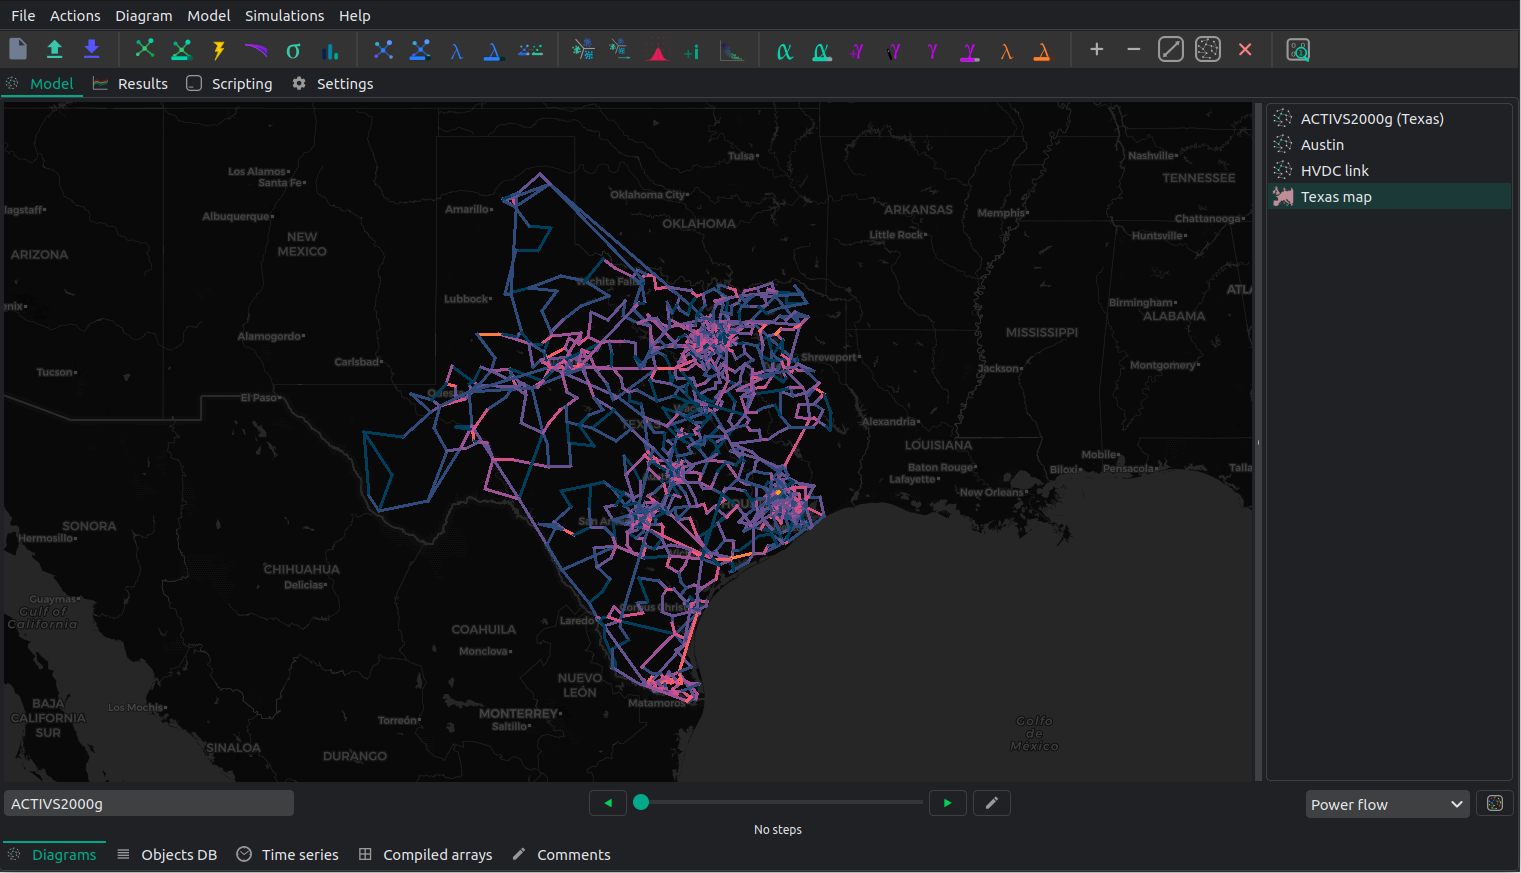
\includegraphics[width=0.8\linewidth]{figures/VeraGrid_main_page.png}
  \caption{VeraGrid main page. \textit{Source}: VeraGrid documentation \cite{veragrid}.}
  \label{fig:VeraGrid_main}
\end{figure}


\subsection{Previous requirements}

Before starting this thesis, it is necessary to have a solid understanding of power system dynamics, numerical methods for differential equations,
and programming in Python. Moreover, this section outlines specific theoretical background on the dynamic simulation of power systems, symbolic formulation and
differential-algebraic equations (DAEs). 

\subsubsection{Dynamic framework in Veragrid}

dfdg
\subsubsection{Differential-Algebraic Equations (DAEs)}

In many dynamic systems, including power systems, their model is not only composed of purely differential equations but also algebraic constraints linking the state
variables. Such systems are naturally represented by differential-algebraic equations (DAEs). Formally, a DAE is an equation of the form: 

\begin{equation}
  F\bigl(\dot{x}(t), x(t), y(t), t\bigr) = 0
\end{equation}


Where $x(t)\in \mathbb{R}^n$ are the differential variables, $y(t)\in \mathbb{R}^m$ are algebraic variables, and the function
 $F$ encodes both the differential and algebraic relations. 
In contrast to an ordinary differential equation (ODE), not all derivatives $\dot{x}$ can be explicitly solved from the system because some variables appear only 
algebraically, that is, without derivative \cite{CasellaDAE}.

One common formulation is the so-called semi-explicit DAE:  
\begin{equation}
\begin{cases}
\dot x = f\bigl(x,\,y,\,t\bigr) \\
0 = g\bigl(x,\,y,\,t\bigr)
\end{cases}
\end{equation} 

Where $f\colon \mathbb{R}^{n+m+1} \to \mathbb{R}^n$ and $g\colon \mathbb{R}^{n+m+1} \to \mathbb{R}^m$. In this form, one treats some variables $x$ as dynamic and others $y$
as constrained by algebraic equations. The condition to solve the DAE is that the partial jacobian $\partial g / \partial y$ is nonsingular so that $y$ can be locally solved as
a function of $x$ and $t$ \cite{CasellaDAE}. If the partial jacobian is singular an iterative process must be done re-casting the problem until it is possible to solve.  

An alternative is the fully implicit form:  

\begin{equation}
f\bigl(\dot{x},\, x,\, y,\, t \bigr) = 0
\end{equation}

With no explicit separation of differential and algebraic parts. In that representation, one works directly with the combined vector $(\dot{x}, x, y)$ and the solver must treat 
the singularity in $\partial f / \partial \dot{x}$. Implicit DAEs are more general and often arise in multiphysics problems and constrained mechanical systems \cite{CasellaDAE}.  

 
In power system dynamics, the network and algebraic constraints ( Kirchhoff's current law, network admittance equations, etc.) naturally provide algebraic equations, 
while generator rotor dynamics, excitation systems, governor control, and other dynamic devices supply the differential equations. Thus a typical formulation is  

\begin{equation}
\begin{cases}
\dot{x} = f(x,\, y) \\
0 = g(x,\, y)
\end{cases}
\end{equation}

Where $x$ includes rotor angles, speed deviations, internal voltages, control states, and $y$ includes bus voltages, phase angles, algebraic currents, and so on \cite{SauerPaiBook}. 
The coupling is strong: every time step, the algebraic network equations must be solved together with the differential updates, typically via Newton-Raphson or other Newton-based 
solvers applied to the full system jacobian.   

This DAE-based representation ensures that the physical constraints of the network are never violated, and that stability and modal analysis reflect the full coupled system behavior,
rather than an oversimplified reduced ODE form.  

\subsubsection{Symbolic framework}

The development of modern power system simulation tools has progressively incorporated symbolic computation to enhance both the analytical transparency and numerical
robustness of dynamic models. A symbolic framework refers to an environment in which the mathematical equations describing a physical system are manipulated symbolically
before numerical evaluation. This approach enables the explicit representation of the differential and algebraic equations governing power system dynamics, allowing the 
automatic derivation of jacobians and linearized models directly from the symbolic expressions.
Such symbolic processing bridges the gap between manual analytical formulation and automated numerical computation, ensuring consistency and reproducibility across 
different analysis tasks \cite{SymbolicHantao}.

In general, a symbolic modeling framework treats system equations as algebraic entities rather than arrays of numbers. Each state variable, parameter, and equation
is represented symbolically and stored in structured form. Once the symbolic system is constructed, operations such as differentiation, substitution, and matrix assembly
can be performed analytically. These expressions can then be compiled into efficient numerical routines to be executed by solvers. 
This two-step process, symbolic formulation followed by numerical evaluation, provides the flexibility to modify models, perform analytical checks
and generate adapted code for various simulation modes without redefining the mathematical structure.

Power systems are naturally suited to this formulation, as their behavior is described by a set of coupled DAEs representing both dynamic components and network constraints.
In this context, generators, exciters, governors, and control systems contribute differential equations, whereas network variables, bus voltages, currents, and algebraic 
constraints from Kirchhoff's laws; are represented algebraically. By expressing these components symbolically, they can be automatically assembled into a unified 
system model and linearized analytically to obtain small-signal representations. This methodology ensures that the global model preserves physical consistency and that 
linearization results, such as eigenvalues and participation factors, are computed with exact analytical derivatives rather than numerical approximations.

The symbolic framework in VeraGrid creates a new set of classes in order to be able to operate in the symbolic framework. To implement the symbolic formulation in practice, VeraGrid defines a minimal hierarchy
 of classes that abstract mathematical entities such as variables, constants, and operators. The main classes are stated below.

\begin{itemize}
  \item \textit{Expr}: Expression is an abstract class that can be used as any expression for a node. Depending of it's nature it can work as many different objects.
  \item \textit{Var}: Variables are stored as their name (string) and their value set as Number (integer, float or complex number) or \textit{Expr}. This allows values stored in
  \textit{Var} to be able to change. Some of the variables can be assigned as \textit{Dynamic variable} which means those variables are part of an other device but are also used in
  the DAEs of the device created.
  \item \textit{Const}: Constants are stored as their name (string) and their value set as Number (integer, float or complex number). Those are frozen parameters of the grid.
  \item \textit{BinOp}: Binary operator stores each possibility of binary operation. The following arithmetic operations are defined: addition, subtraction, multiplication, division and exponentiation.
  \item \textit{Func}: Functions store each individual function possible that can be part of an equation: sinus, cosinus, tangent, logarithm, real or imaginary parts among others.
\end{itemize}

All these elements are unified to create \textit{Blocks}, a set of differential and algebraic equations and stated variables that form the symbolic representation of the DAEs of each
element. Blocks also include a set of initializing variables and equations and fixed variables and equations that help initialize the DAEs and allow a fastest solution. All variables in a Block are stored as 
children of that Block in order to allow recursivity. This recursive structure means that each block can contain child elements (either variables or 
other blocks) allowing a hierarchical representation of the power system. Such a design enables complex devices and networks to be constructed from smaller symbolic components 
while maintaining full analytical traceability.


Moreover, parameters are also defined as the variables or constants affected by events that can be added to the grid.

VeraGrid's version of the symbolic framework includes three different types of elements in the grid: buses, injections and branches. Injections include all types of elements
that contribute actively to the system: generators, loads, batteries, shunts... Branches include the devices that connect buses: lines, transformers, converters... 

One example is the synchronous generator model. First, all variables are assigned to class \textit{Var}. The voltage module and angle are stated as dynamic variables as they are also 
considered on the bus model. Then, the block is created by stating all the state and algebraic equations and variables and the initialization and fixed equations and variables. The differential
and algebraic equations of the synchronous generator are stated below.

\begin{equation}
\begin{cases}
\delta = 2\pi f\,(\omega - \omega_{ref}) \\
\omega = \dfrac{\Gamma_m - \Gamma_e - D(\omega - \omega_{ref})}{M}
\end{cases}
\label{eq:diff_eq_gen}
\end{equation}

\begin{equation}
\begin{cases}
\psi_d - (R \cdot i_q + v_q) = 0 \\
\psi_q + (R\cdot i_d + v_d) = 0\\
0 - ( \psi_d + X \cdot i_d - v_f ) = 0\\
0 - (\psi_q + X \cdot i_q) = 0 \\
v_d - (V_m \cdot \sin(\delta - V_a)) = 0\\
v_q - (V_m \cdot \cos(\delta - V_a)) = 0\\
\Gamma_e - ( \psi_d \cdot i_q - \psi_q \cdot i_d ) = 0\\
P_g - (v_d \cdot i_d + v_q \cdot i_q) = 0\\
Q_g - (v_q \cdot i_d - v_d \cdot i_q) = 0 \\
\Gamma_m - (\Gamma_{m0} + K_p(\omega - \omega_{ref}) + K_i \cdot e_t) = 0\\
2\pi f \cdot e_t - \delta = 0
\end{cases}
\label{eq:alg_eq_gen}
\end{equation}

Where:
\begin{itemize}
  \item $\delta$: Rotor electrical angle with respect to the synchronous reference frame [rad].
  \item $\omega$: Rotor angular speed [rad/s].
  \item $f$: Nominal electrical frequency [Hz].
  \item $\Gamma_m$: Mechanical torque applied to the rotor [p.u.].
  \item $\Gamma_{m,0}$: Initial mechanical torque reference [p.u.].
  \item $\Gamma_e$: Electromagnetic torque produced by the generator [p.u.].
  \item $D$: Damping coefficient representing mechanical damping effects [p.u.].
  \item $M$: Inertia constant of the rotor [p.u.·s].
  \item $\psi_d$: d-axis stator flux linkage in Park reference frame [p.u.].
  \item $\psi_q$: q-axis stator flux linkage in Park reference frame[p.u.].
  \item $R$: Stator winding resistance [p.u.].
  \item $X$: Stator synchronous reactance [p.u.].
  \item $v_d$: d-axis stator voltage component in Park reference frame [p.u.].
  \item $v_q$: q-axis stator voltage component in Park reference frame [p.u.].
  \item $i_d$: d-axis stator current component in Park reference frame [p.u.].
  \item $i_q$: q-axis stator current component in Park reference frame [p.u.].
  \item $v_f$: Field excitation voltage [p.u.].
  \item $V_m$: Magnitude of the terminal voltage phasor [p.u.].
  \item $V_a$: Angle of the terminal voltage phasor with respect to the reference frame [rad].
  \item $P_g$: Active electrical power delivered by the generator [MW].
  \item $Q_g$: Reactive electrical power delivered by the generator [Mvar].
  \item $K_p$: Proportional gain of the speed governor control [-].
  \item $K_i$: Integral gain of the speed governor control [-].
  \item $e_t$: Integral term of the governor controller, representing the accumulated speed error [rad/s].
\end{itemize}

It should be noted that the DAEs representing each element and device in the network can be simplified or extended depending on the desired level of modelling accuracy. 
A trade-off must therefore be established between computational complexity and numerical accuracy. In practical applications, simplified formulations are often used for 
large-scale steady-state or RMS simulations, whereas more detailed dynamic representations are required for transient and small-signal stability studies. The flexibility 
of the symbolic framework allows the modeller to adapt the formulation of each component accordingly, preserving analytical consistency while optimizing computational 
performance.




\newpage